% will smith citation 

\documentclass[10pt,letterpaper]{article}
\usepackage{graphicx}
\usepackage{cogsci}
\usepackage{pslatex}
\usepackage{apacite2}
\usepackage{subfigure}
\usepackage{amsmath}
\usepackage{amssymb}
\usepackage{tikz}
\usepackage{marvosym}
\usepackage{wasysym}
\usepackage{times}
\usepackage{epsfig}
\usepackage{tabularx}
\usepackage{enumitem}
\usepackage{sidecap}
\usepackage[titletoc,toc,title]{appendix}


\usetikzlibrary{decorations.pathreplacing,calc}
\title{Discovering the Signatures of Joint Attention in Egocentric Video}

\author{{\bf Guido Pusiol}\\ 
\texttt{guido@cs.stanford.edu} \\
Department of Computer Science\\
Department of Psychology \\
Stanford University
  \And {\bf Laura Soriano} \\ 
\texttt{lsoriano@stanford.edu} \\
Department of Psychology\\
Stanford University 
\And {\bf Li Fei-Fei} \\
\texttt{feifeili@stanford.edu} \\
  Department of Computer Science\\
Stanford University 
\And {\bf Michael C. Frank} \\ 
\texttt{mcfrank@stanford.edu} \\
  Department of Psychology\\
Stanford University}
  
\newcommand{\argmax}[1]{\underset{#1}{\operatorname{arg}\,\operatorname{max}}\;}
\begin{document}
\maketitle

\begin{abstract}

\textbf{Keywords:} 
Joint attention; computer vision; child development; social cognition. 
\end{abstract}



\section{Introduction}

How do young children begin learning the meanings of words? Across cultures, early vocabulary includes names for people, simple social routines, animals, and objects \cite{tardif2008}, suggesting that the earliest words are learned through interaction and play with others \cite{bruner1985}.  Identifying a caregiver's intended referent is a critical part of learning meaning within these interactions, and this identification is often accomplished through \emph{joint attention}.

Joint attention describes the situation when both child and caregiver are attending to the same thing and when both know that the other is attending to it \cite<for the remainder of the paper we will talk informally about joint attention---JA---as both the phenomenon and the period of time during which it happens;>{carpenter2011}.  A typical example of JA is a situation where an adult and child are playing with a toy and the infant alternates gaze between the adult and the toy \cite{carpenter1998}. 

The capacity for JA gradually develops over the first two years of life and usually begins to emerge between 9 and 12 months of age \cite{morales2000}, coinciding with the beginnings of language learning. In addition, both the skills that enable JA (e.g. pointing, following a caregiver's gaze to a distal target) and the amount of time that children spend in JA with their caregivers are strong predictors of children's early vocabulary growth \cite{carpenter1998,brooks2008,tomasello1983}. 

But how do children \emph{know} that they are in joint attention with a caregiver? From an external perspective, joint attention has typically been defined by a sequence of events: (1) one member of the interaction (child or caregiver) directs the other member’s attention to an object, (2) both members focus visually on the object, and (3) the child indicates awareness of the caregiver  \cite{tomasello1986}. 

Previous work has typically used children's gaze as the main indicator of JA, but, from the perspective of both the child and the data analyst, this method has several issues. First, gaze is neither necessary nor sufficient for JA. It is possible to attend jointly through the hands---as with a child reading a picturebook on a parent's lap---or for the child to follow gaze to a distal target and then signal awareness by moving towards it or reaching for it. Indeed, eye-tracking studies investigating signals to reference find that manual signals are far more effective than gaze in manipulating young children's attention \cite{yurovsky2013}. Second, young children may not have perceptual access to their caregiver's gaze most of the time. Recent studies using head-mounted cameras and eye-trackers suggest that children are more often looking at the objects in front of them than at the faces of their caregivers \cite{smith2011,franchak2011,frank2013}. Third, parents most often look at their children, not at the object they are talking about \cite{frank2013b}. Thus, gaze alone is at best a noisy cue for the identification of JA, either for the child or for the researcher attempting to identify JA in a large dataset.

The goal of our current work is to discover other signals of joint attention. There are two purposes to this investigation. The first is data analytic: A better understanding of how to extract JA episodes from video could be a powerful tool for analyzing video corpora. The second is psychological: The unsupervised extraction of JA episodes from video could give hints regarding robust cues that children might use in addition to, or even in lieu of, gaze. 

We use two data sources to gain information about the social interaction between child and caregiver: head-mounted and fixed camera videos. Our approach is unsupervised discovery. We hypothesized that the most effective strategy for capturing JA would be the extraction of high-level, semantic features that correspond relatively closely to the kinds of constructs described in prior work manually coding joint attention \cite<e.g.>{tomasello1983}. Of course, the challenge is that many such features can be extremely difficult to extract in an automated fashion. To compromise, we identified three features that we could extract with relatively high accuracy in an automated fashion; we hypothesized that each of these might have some relationship to JA: (1) caregivers' faces in the egocentric camera, (2) objects that were in motion due to being actively manipulated, and (3) periods of time during which the child's attention was relatively static. 

The plan of the paper is as follows. We begin by describing our dataset, and then we describe how we use computational methods to extract semantic features from these data. We then examine the correlations between these features (and higher-level clusters of these features) and hand-coded joint attentional episodes. Our results suggest that there are a number of redundant perceptual cues to JA, and that some of these may be more readily accessible to children than gaze. In future work, some of these cues could form a robust basis for the automatic detection of joint attentional episodes.


\section{Dataset}

\subsection{Videos}

We make use of a dataset of in-lab caregiver-child play sessions initially described in \citeA{frank2013}. In this dataset, parents were invited to play one-on-one with their children on the floor of a friendly, colorful room. The children wore a small head-mounted (egocentric) camera that captured their approximate visual experience, and a tripod-mounted camera captured the third-person perspective from one corner of the room. Child and caregiver played with a set of toys organized into pairs, with each pair containing a known object (e.g. a ball) and a novel object (e.g. a yellow feather duster). The novel objects were clearly labeled so that parents knew what to call them (e.g. the duster was a ``zem''). For purposes of the current study, we chose a set of FIXME videos containing three eight-month-old children and three sixteen-month-old children. Each video was between FIXME and FIXME minutes long. 

\begin{figure}[t]
     \begin{center}
        % \subfigure[todo]{%
           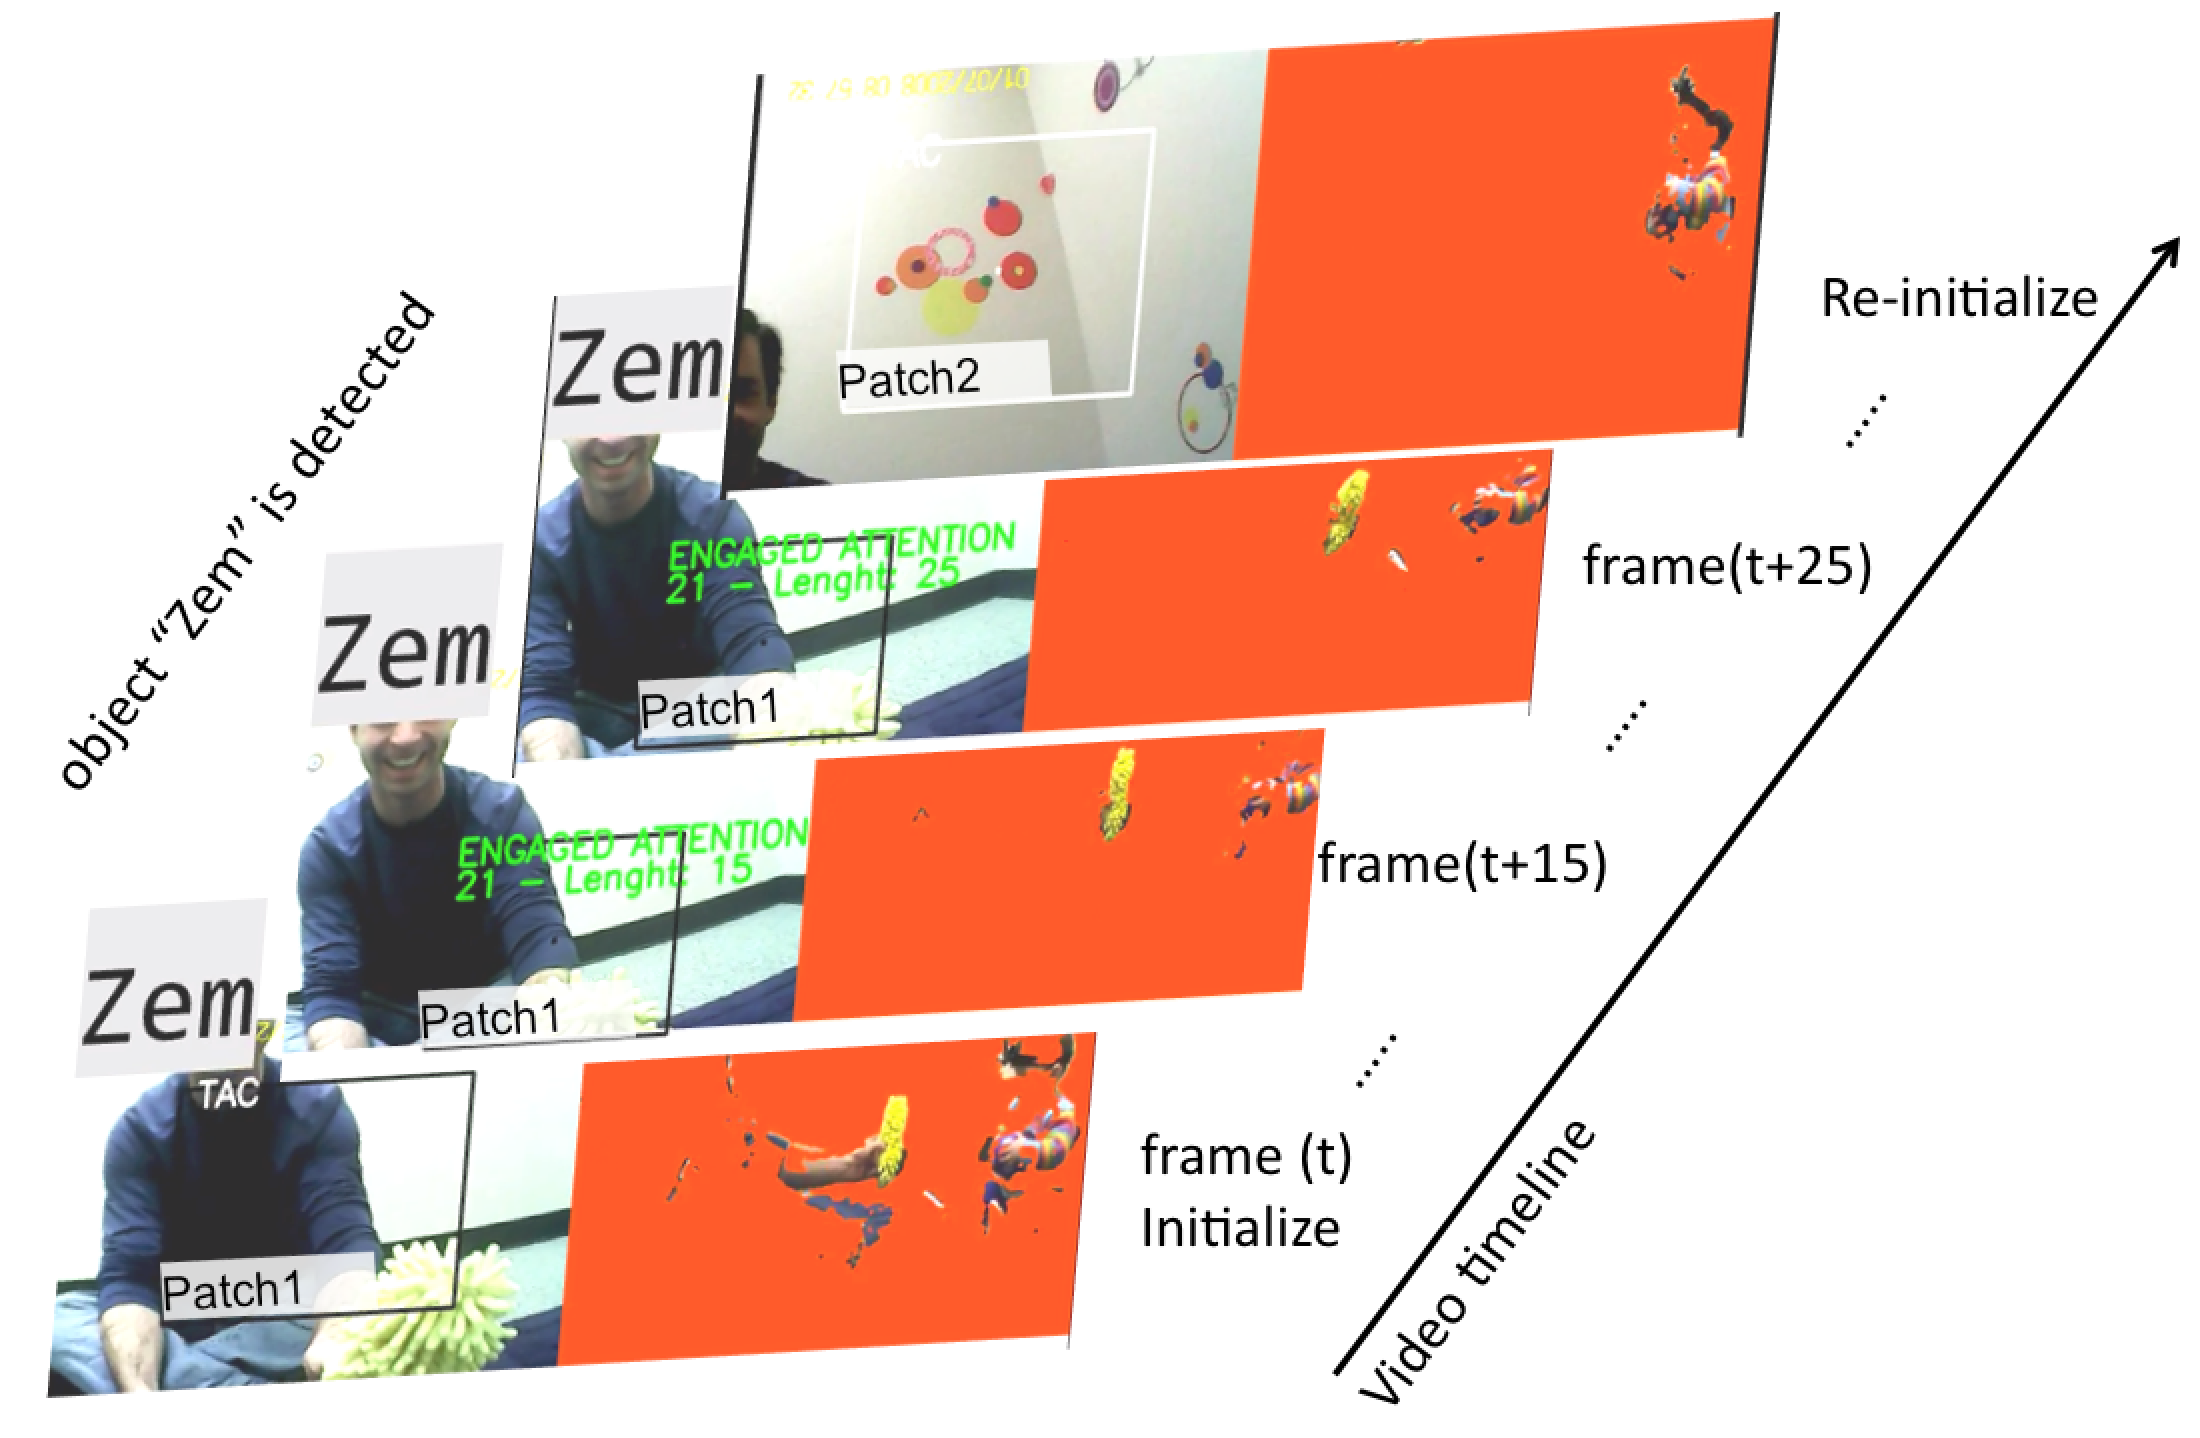
\includegraphics[width=1\linewidth]{Image/cogsci} 
           % }
          \end{center}
    \caption{An example of our synchronized dataset: The left side of each panel shows the egocentric video, while the right side shows the motion-filtered 3rd person video. The rectangle in the middle of the egocentric camera shows the attention chunk tracker, while the label ``zem'' indicates that the object detector has found the yellow feather duster in the 3rd person video.}
   \label{fig:main}
\end{figure}

\subsection{Annotation of Joint Attention}

We used the DataVyu software package \cite{adolph2012} to annotate periods of time during which child and caregiver were in joint attention. Joint attention was defined if it satisfied the criteria given by \cite{tomasello1983}. First, the interaction had to begin with either parent or child initiating. For example, a parent could hold up an object and label it, or a child could bring an object over the parent. Second, both members were required to focus on the object in JA for at least 3 seconds; we allowed this period to include brief glances away. Third, at some point during the interaction the child was required to display some overt behavior towards the parent to show that he or she acknowledged the interaction.

\section{Defining Semantic Features}

We describe automatic and semi-automatic methods for creating high-level semantic features capturing caregivers' faces and episodes of static attention (``attention chunks'') from egocentric video and moving objects from the third-person video.

%%%%%% FIGURE FACE DETECTION

\subsection{Face Detection}

Traditional off-the-shelf face detection algorithms \cite<e.g.>{viola2001} fail at detecting parent faces in the kinds of egocentric video that we collected. Face detectors work accurately when the test dataset has low variance from the training dataset and the distance between the camera and the face is \textgreater 1 meter (e.g. Facebook-style pictures). From the egocentric perspective, however, many other face configurations are prevalent. Faces appear partially occluded or cropped, blurred by motion, and with large size and texture variability making detecting them very challenging (Figure \ref{fig:faces}). 

We addressed the problem using a semi-automated adaptive algorithm \cite{kalal} that makes use of minimal user input for initialization (selecting one example face per video). The algorithm uses new pixel patches in the trajectory of an optical-flow based tracker to train and update a face detector. The optical flow tracker and the face detector work in parallel. If the face detector finds a location in a new frame exhibiting a high similarity to its stored template, the tracker is re-initialised on that location. Otherwise, the tracker uses the optical flow to decide the location of a face in the new frame. 

The primary advantage of the algorithm is the use of motion for face detection: Following the movement of the pixels that define a face it is possible for the algorithm to adapt to new morphologies (i.e. different face poses). More broadly, this method allows for a face that is partially occluded or poorly lit to be tagged as a face by virtue of its relationship with previous frames where the face information was clearer. 

\begin{figure}[t]
          \subfigure[Motion blur]{
             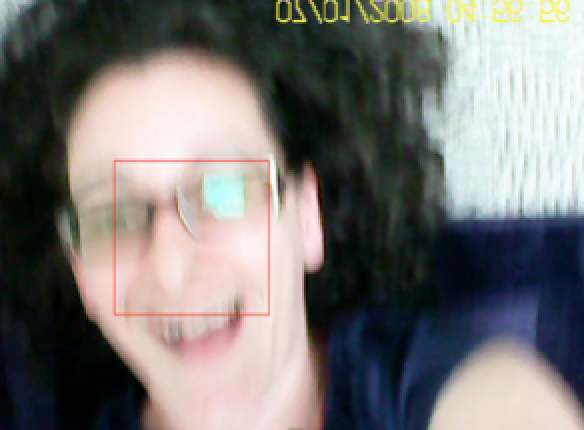
\includegraphics[width=1in,height= 1in]{Image/a}
             }    
            \subfigure[Partial occlusion]{
            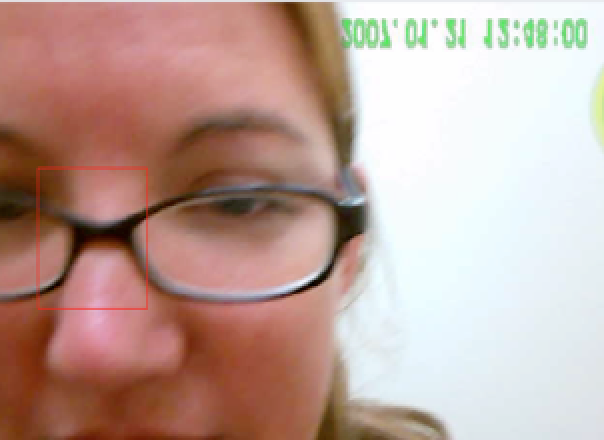
\includegraphics[width=1in,height= 1in]{Image/c} 
            }
             \subfigure[Low texture]{          
             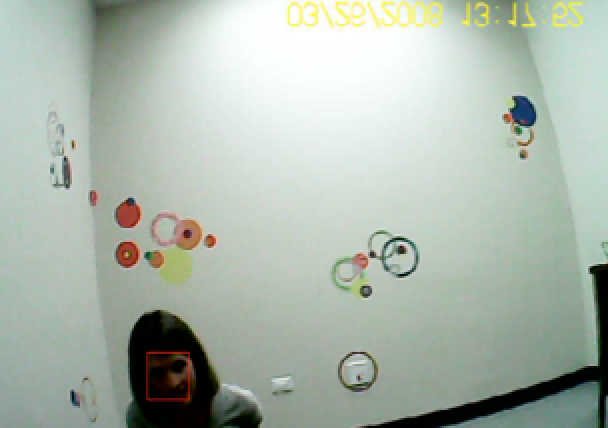
\includegraphics[width=1in,height= 1in]{Image/d} 
             }
    \caption{Three examples of challenging faces for traditional detectors.}
\label{fig:faces}
\end{figure}

\subsubsection{Evaluation}

As part of an ongoing study following \citeA{frank2013}, we evaluated this face detector using a set of 37 egocentric videos gathered in the circumstances described above (with ages ranging from 8 -- 16 months).  Our evaluation compares automatically detected faces with human ground truth annotations over a sample of both high face-density and randomly selected frames. We found that our algorithm had precision of FIXME and recall of FIXME, achieving a relatively high level of accuracy in this challenging dataset. 

 % .92 and recall of .99; true Negatives = 93; accuracy = 96 outperform the state of the art \cite{dpmface} due to the active-learning stage of the algorithm.\\



%%%%%% ATTENTION MOTION  ATTENTION CHUNKS
\subsection{Detecting Episodes of Static Attention}

One important aspect of joint attention is that it should be (relatively) static if the child is focused on a single object. Congruent with that, previous work has found that episodes where a single object dominates the field of view (and hence the view field is static) are predictive of word learning \cite{smith2011,pereira2013}. We attempted to identify such moments of fixed attention (``attention chunks'') in an automated way. Our strategy is to track a large-scale region of the video (e.g. background texture) across frames; if this texture remains in a relatively static location, we can infer that the child's head has not moved significantly. If the texture deforms substantially, then the head is likely to be in motion. This approach is supported by prior experimental work indicating that eye gaze and head pose are typically coupled \cite{yoshida2008}. % Land1,Pelz


% The attention chunks capture the segments of video of a child engaged visually to a concept. They are extracted of the head camera
% . The concept can be a concrete object (face, toy, etc.) or an abstract texture captured by the camera when the child's gaze is attending to an off-scope object (e.g. the child is handling a toy near his chest). The ideal case is to have eye trackers to understand the gaze of the baby, but such a configuration is very hard to achieve in uncontrolled environments. Thus, we use the head-cam information as a gaze estimator. Our 


The algorithm is initializes by modeling a pixel-texture patch ($P_{i}$). For each new frame the algorithm will seek for a similar patch to the one observed in the previous frame. If the patch is matched, a new point is added to the patch trajectory. If the matching is not achieved, a new patch ($P_{i+1}$) is learned and the tracking algorithm is re-initialized. The base algorithm used for tracking is a version of a ``tracking by detection'' algorithm \cite{kalal}. A chunk is defined as the video segment defined by the $start_{P}$ and $end_{P}$ frames of the tacked patch trajectory.

% The figure \ref{fig:chunk} describes the basics of an attention chunk computation.\\
% \begin{figure}[h]
% \begin{center}
%         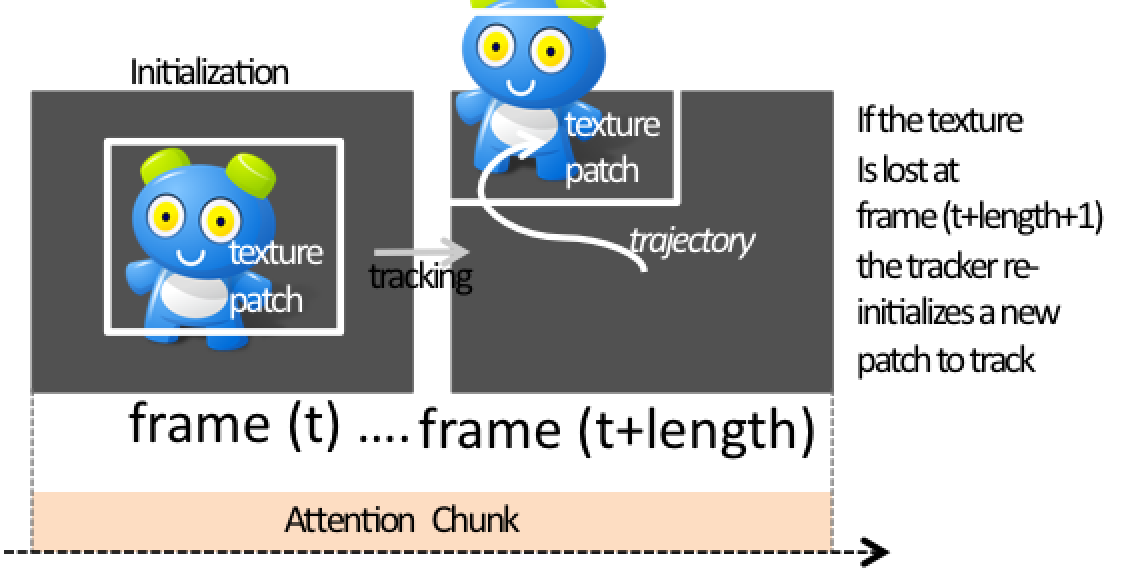
\includegraphics[width=0.5\linewidth]{Image/Attchunk}      
%           \end{center}
%     \caption{Attention chunk computation.}
%    \label{fig:chunk}
% \end{figure}

\subsubsection{Evaluation}

\begin{figure}[t]
\begin{center}
        % \subfigure[Average attentional chunk duration for children at 8, 12, and 16 months.]{           
        %    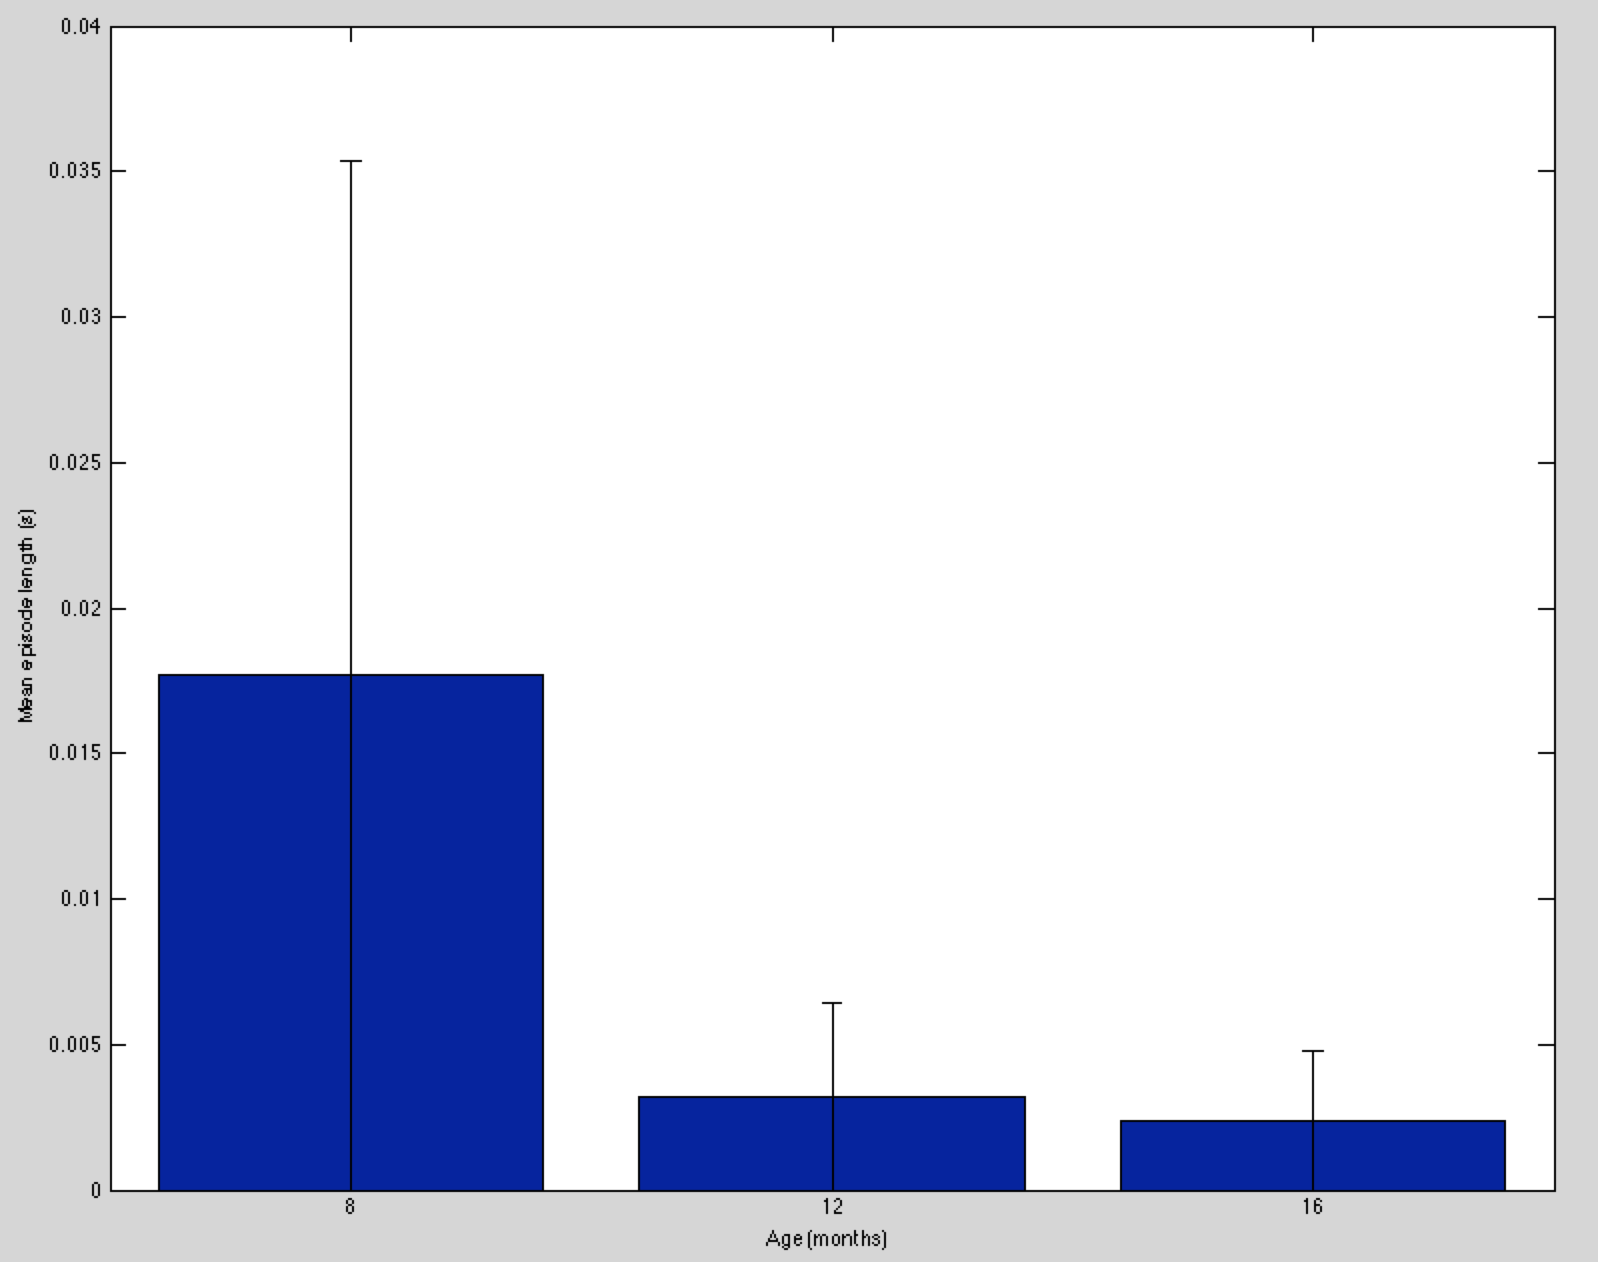
\includegraphics[width=0.45 \linewidth]{Image/log3}
        %    \label{fig:duration}
        %    }
        %    \subfigure[Duration of the attentional chunks distributed in buckets of 10ms and displayed in log scale (i.e. longer chunks appear to the right).]{%
           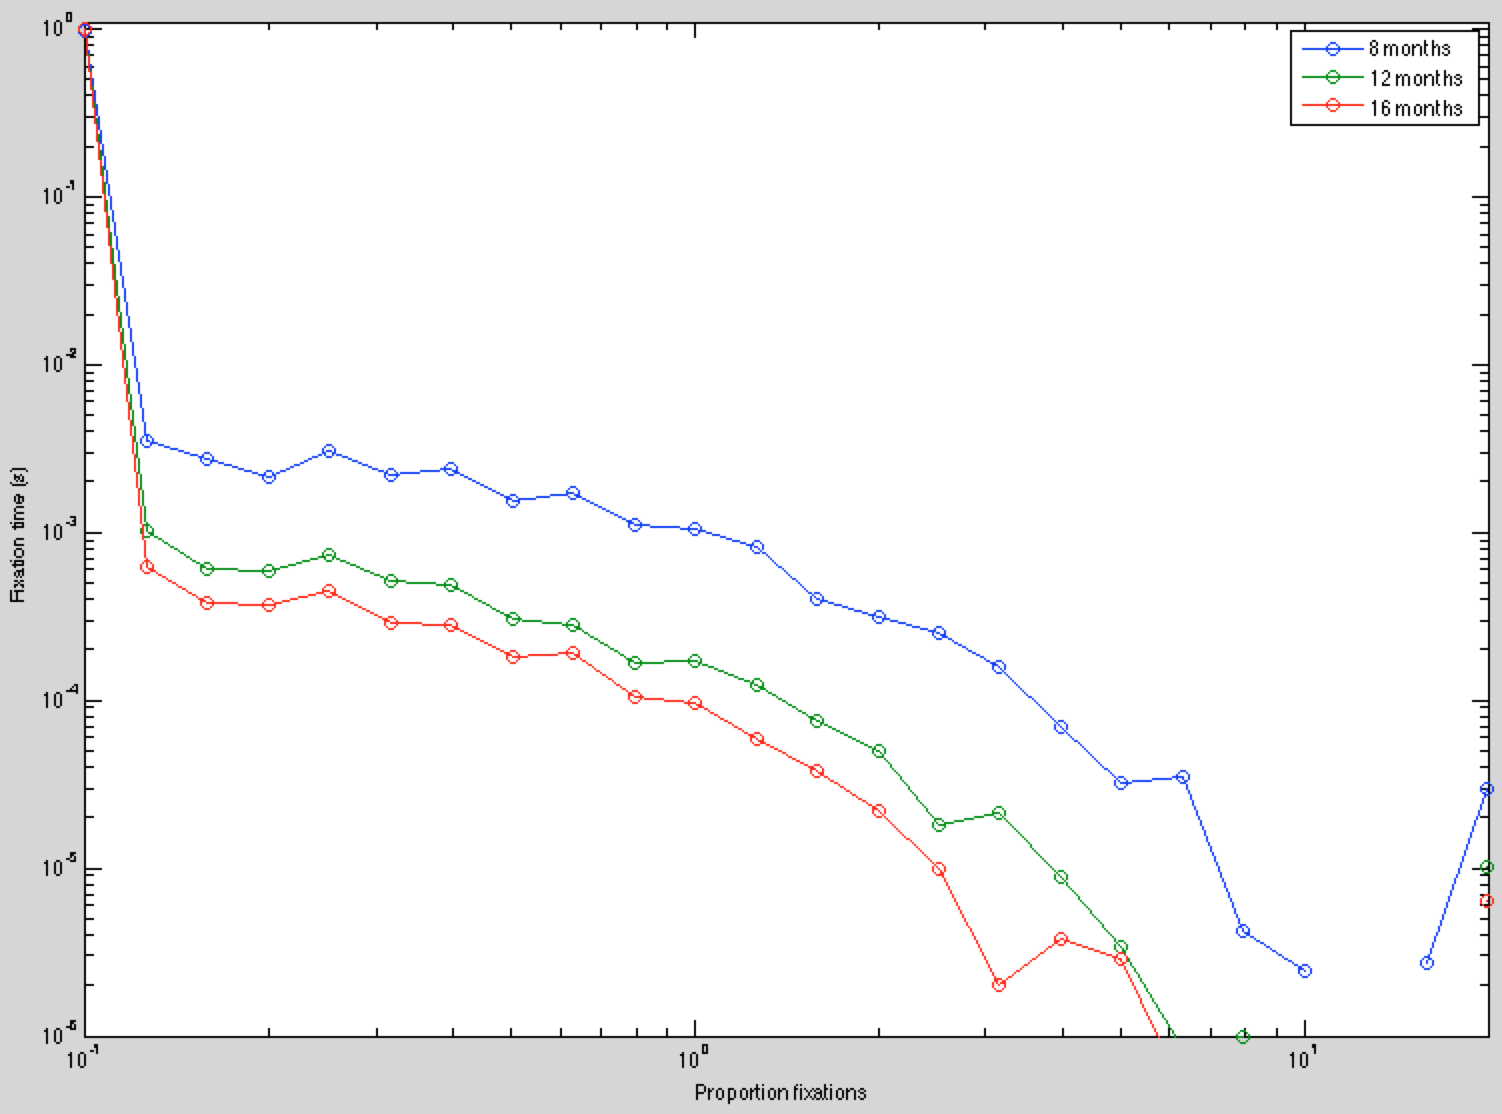
\includegraphics[width=3.4in]{Image/log2}    \label{fig:buckets}
            % }
\caption{The distribution of attention chunk lengths for 8, 12, and 16 month old children. FIXME}
\label{fig:chunks}
\end{center}
\end{figure}

We evaluated the attention chunk method using the larger dataset of 37 egocentric videos. Average chunk duration is shown in Figure \ref{fig:chunks}. The method yielded a distribution that included many very short chunks (presumably while the head was in motion) as well as some longer episodes of attention. We additionally found that the younger children in the sample (8 months) attended somewhat longer on average. We speculate that this pattern is due to the older children's greater autonomy and mobility. 

% The figure \ref{fig:buckets} depicts the temporal duration of the chunks distributed in buckets of 10ms in a log scale. The graph shows that the decay is proportionally symmetric among the different groups, most of the attention chunks are of short duration and there are not "distractors" (i.e. a TV) that interfere with our guided attention towards new objects. 

\subsection{Detection and Tracking of Moving Objects}

As described in our earlier work, the vertical field of view of the head-mounted camera is relatively limited ($\sim40^\circ$ visual angle). Thus, to be able to capture faces high in the visual field, the camera must be at a relatively high angle; this angle in turn precludes capturing the objects that the child is holding. Because of this, we made use of the 3rd person static video to detect the objects that were being handled by the child and the caregiver. 

% We aim at exploring cues of joint attention expressed by hand interactions. The detection of objects being moved even when they are not fully in the visual scope of the children could indicate that the joint attention is established.

% From a computer vision perspective, the objects are highly deformable making them hard to detect and track. The deformations are due to the changes of positions and hand-object occlusions that the object can take while is being manipulated. 

Detection of deformable objects in a colorful, dynamic context is currently an open challenge for computer vision algorithms. Our data contained a wide variety of deformations due to the child-friendly nature of the objects and the consistent occlusion of parts of the objects by caregivers' and children's hands.  To circumvent this difficult challenge, we made use of motion as a convenient, psychologically-inspired ``filter.'' Objects that are in motion are more likely to be attended by the child and/or caregiver; in addition, considering only those pixels that are in motion significantly constrains the object-detection problem (Figure \ref{fig:objects}). 

%For that we make extensive use of local binary patterns as texture descriptors.
\begin{figure}[t]
     \begin{center}
          \subfigure[Object of interest (marked by the yellow square) could be confused with other objects with similar textures and colors (marked in red). Considering only pixels that are in motion effectively filters these distractors.]{
        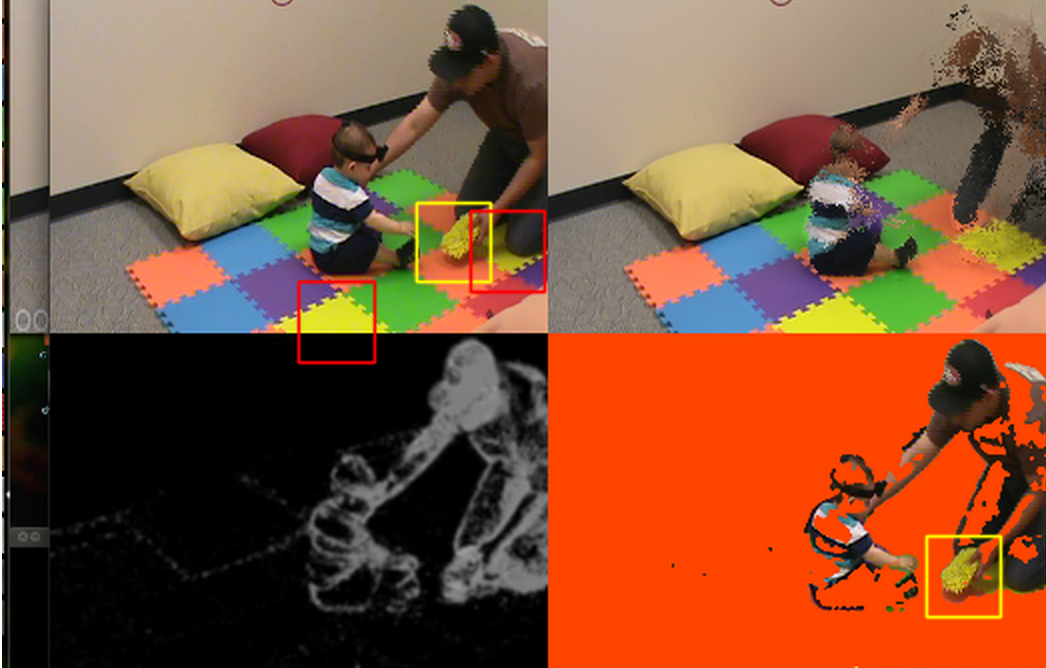
\includegraphics[width=0.8\linewidth]{Image/Zem}}
        \subfigure[Objects of interest are being handled and are therefore moving (yellow square). Unattended objects (red square) are filtered out.]{
        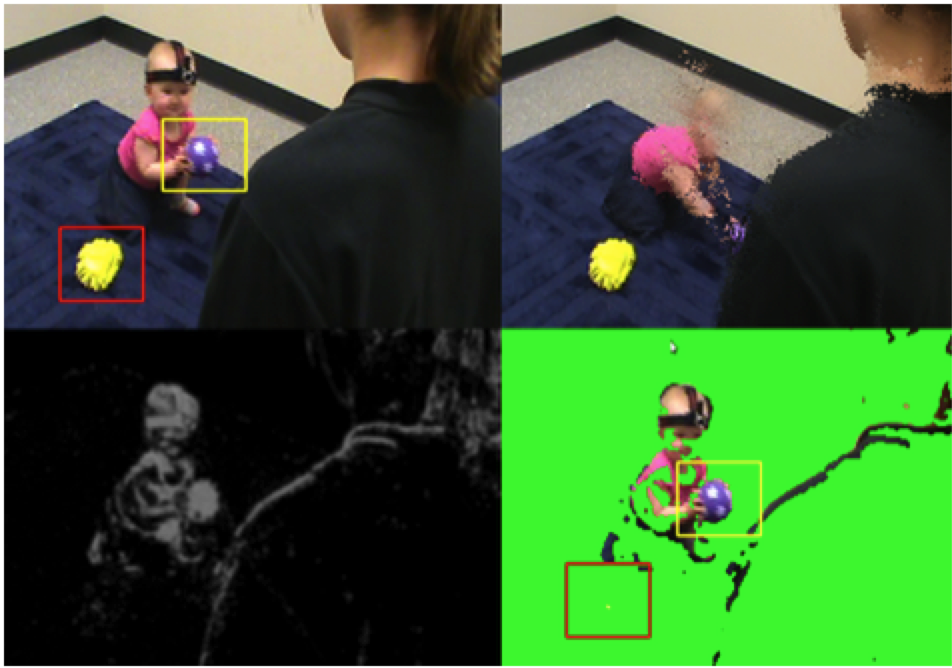
\includegraphics[width=0.8\linewidth]{Image/four}}
        \end{center}
    \caption{Foreground computation. In each image, top left shows original color frame, top right shows  background model color vector, bottom left shows foreground weights, bottom right shows foreground extraction (orange/green pixels correspond to the background mask). (a) shows the problem of texture and color overlap between the object of interest and other objects. (b) shows how this method can also filter out unattended objects.}
   \label{fig:objects}
\end{figure}

\subsubsection{Foreground Modeling}

The goal of foreground modeling is to construct and maintain a statistical representation of the scene so that new information (e.g. due to motion) can be accurately extracted. We chose to utilize both texture information and color information when modeling the background. We follow the approach of \citeA{odobez1}, which exploits the Local Binary Pattern (LBP) feature as a measure of texture because of its good properties \cite{Halika}, along with an illumination invariant photometric distance measure in the RGB space. However, we modified the LBP algorithm to include a larger amount of texture from neighboring pixels. In brief, this approach computes summary statistics over the static background and searches for local deviations to those summary statistics (due to motion).

% POSSIBLY ADD MORE SUMMARY?

% The background model ${{B}^{t}(x)}$ of the pixel $x$ at the time $t$ is represented by a list of modes $\{ {m}^{t}_{k}(x)\}_{k=1\dots K}$. The modes register historic information of 7 features of the pixel's color and surrounding texture. 
% ${m}^{t}_{k} = \{I ,\hat{I},\breve{I}, {LBP}_{k}, w,  \hat{w}, P \}$. 
% Where ${I}$ represents the average $RGB$ image vector. $\hat{I}$ and $\breve{I}$ are the maximal and minimal $RGB$ image vectors. {LBP} is the vector of local binary patterns computed at this mode.\\
% The background model can learn up to $K^{max}$ different modes. For each new $I^{t}$ and $LBP^{t}$ a new mode is computed $m^{t-1}_{k}$ and the algorithm seeks to which learned mode $m^{t-1}_{k}$ the new mode maps to. The mapping is achieved by thresholding a distance (i.e $\tilde{k} = \underset{{k}}{\arg\min} ~ D(m^{t-1}_{k},m^{t}_{k})$). 1) If the new mode cannot be mapped to any of the learned ones and there is still space in the buffer ($K $\textless$ K^{max}$), then a new mode is initialized. 2) If there is a matched mode $m^{t-1}_{\tilde{k}}$, its representation is updated as follows:
% \begin{equation}
%    \begin{cases} 
%      \breve{I}_{\tilde{k}}^{t} = min (I^{t}, (1 + \beta) \breve{I}_{\tilde{k}}^{t-1}), \\
%      \hat{I}_{\tilde{k}}^{t} = max (I^{t}, (1 - \beta) \hat{I}_{\tilde{k}}^{t-1}), \\
%      {I}_{\tilde{k}}^{t} = (1 + \alpha) {I}_{\tilde{k}}^{t-1} + \alpha	{I}^{t}, \\
%      {LBP}_{\tilde{k}}^{t} = (1 + \alpha) {LBP}_{\tilde{k}}^{t-1} + \alpha	{LBP}^{t}, \\
%      (*)w^{t}_{\tilde k}= (1 - \alpha^{i}_{w}) {w}_{\tilde{k}}^{t-1} + \alpha^{i}_{w},\\ ~~~ ~~~ ~~~ \alpha^{i}_{w}=\alpha_{w}(1+\tau\hat{w}^{t-1}_{k}) \\
%      \hat{w}^{t}_{\tilde{k}} = max (\hat{w}^{t-1}_{\tilde{k}}, w^{t}_{\tilde{k}})\\
%      L^{t}_{\tilde{k}} = 1+ max \{L^{t-1}_{k}\}_{k=1,\dots,K, k \neq \tilde{k}},\\ ~~~ ~~~ ~~~ if~~ L^{t}_{\tilde{k}}~=~0~and~T_{bw} $\textless$\hat{w}_{\tilde{k}}^{t} \\
%    \end{cases} 
% \end{equation}

% where $\beta \in [0,1)$ is the learning rate of the min and max color vectors and $\alpha \in [0,1)$ is the learning rate of the color and texture information. The non matching modes of the previous model are assigned to the new model (i.e. $m^{t}{k}:=m^{t-1}{k}$ ) but their weights are decreased according to (*).
% \\
% After the update step, all nodes are sorted decreasingly according to their weight. And the background modes are the first $B^{t}$ modes that satisfy:
% \begin {equation}\sum_{k=1}^{B^{t}} w_{k}^{t} / \sum_{k=1}^{K^{t}} w_{k}^{t} < TB \end{equation} where $TB  \in [0,1]$ is the background threshold.
% Due to the use of both color and texture in this computation, the chances that moving foreground objects generate a consistent mode over time (and hence are filtered out) is quite small.

\subsubsection{Object Tracking}

We used the extracted foreground pixels as the input to object-tracking algorithms. 
% We are interested in detecting a tracking a set of objects (i.e. toys) components of triad when the parents and children are engaged in a JA episode. In particular the toys are being manipulated. The detection and tracking objects is performed over the foreground image. 
We experimented with a number of appearance-based object detectors with relatively poor results \cite{TLD}. Our solution was to detect and track objects by their color and relative size. We modified the cam-shift algorithm \cite{bradsky}, a specialization of the mean-shift algorithm.
 % \cite{Meer2002}
Mean shift is a non-parametric technique that climbs the gradient of a probability distribution to find the nearest dominant mode (peak). In our case, this distribution is based in color values. The algorithm is initialized by selecting a region containing the object of interest and building a color histogram over the region. In a new frame, the algorithm will match the region's size and the peaks of the color distribution using both mean-shift and euclidean distance metrics. Figure \ref{fig:track} shows examples of the detection and tracking of two different objects.

\begin{figure}[t]
     \begin{center}
        \subfigure[``Manu'' detected.]{
           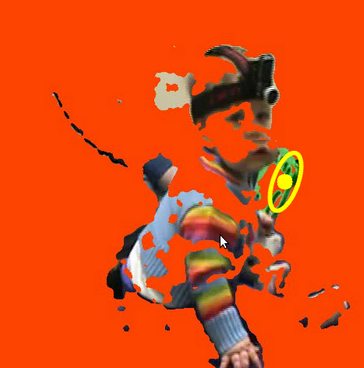
\includegraphics[width=0.4\linewidth]{Image/g2}
           \label{fig:tracking} 
           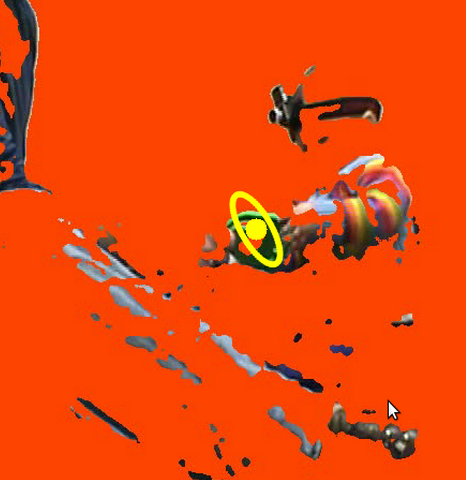
\includegraphics[width=0.4\linewidth]{Image/g4}
            }
          \subfigure[``Zem'' detected.]{
           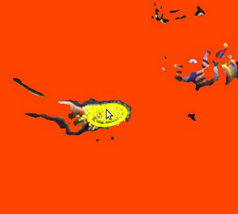
\includegraphics[width=0.45\linewidth]{Image/z1}

          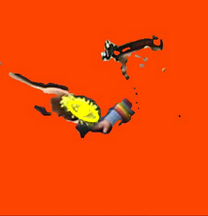
\includegraphics[width=0.4\linewidth]{Image/z2}
           \label{fig:tracking} }
         
    \end{center}
    \caption{Four examples of object detections within the foreground of the static, 3rd person video.}
   \label{fig:track}
\end{figure}


\section{Feature Aggregation}

In the previous sections we detected and computed features (faces, objects, etc.) from different cameras. The goal of the next stage is to merge and prune these features into a single matrix describing the detected features for each video frame. This aggregation required a number of decisions to be made. First, we synchronized frames across the cameras (which had different frame rates). Next, we calculated six features for each frame $f$ (all normalized to the same interval based on the observed maximum and minimum): 

% {\bf 4.1. Synchronization.} We calculate the bijective function mapping each frame of the fixed camera to the head mounted camera (i.e. figure \label{fig:main} ). When the inter camera frames can be mapped, the detected features and video attributes of both cameras can also be mapped together.\\

% {\bf 4.2. Features definition.} We calculate 6 features for each video $frame_{t}$. 
\begin{enumerate}[noitemsep]
\item Chunk length: The number of frames in the attention chunk containing $f_{t}$.
\item Chunk speed: The average speed of the attention chunk's trajectory. 
\item Face speed: The speed ($L_{2}$ norm) of the face position at $f_t$ and $f_{t-1}$. 
\item Face size: The diagonal of the bounding box for the face (a proxy for distance between parent and child).
\item  Object speed: The speed ($L_{2}$ norm) of the detected object's position at $f_t$ and $f_{t-1}$.    
\item Object size: The diameter of the ellipse FIXME bounding the detected object.
\end{enumerate}
% The lack of detection is replaced by the 0 value.\\ 

Because object and face features were computed frame by frame, we experimented with using the attention chunks as a way to propagate features across larger ranges of time. Using this method, all those objects and faces detected in a single video frame that fell within an attention chunk were propagated to all of the frames of the chunk. Assuming that the attention chunks have some value as indicators of the child's attention, this step should improve the quality of detections. We report results both with and without this propagation step. 

\section{Evaluation}


\begin{SCfigure*}
  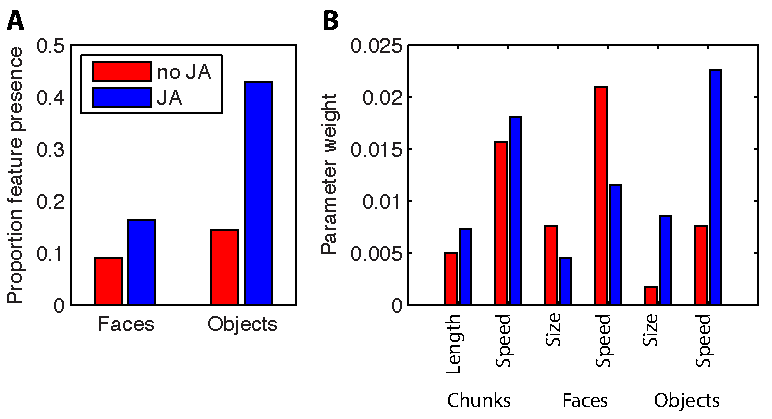
\includegraphics[width=4.5in]{Image/classifier2.pdf} 
  % \begin{center}
  \caption{(A) Proportion of faces and objects detected both in and out of joint attentional episodes. (B) Mean parameter weights on each of the six features we considered for the JA and non-JA categories in the Naive Bayes Classifier. Legend is as in (A).  \label{fig:main}}
  % \end{center}
\end{SCfigure*}

% \begin{table}[t]
% \centering
% \begin{tabular}{ccc|cc|cc}
% & & &\multicolumn{2}{c}{Face} & \multicolumn{2}{c}{Object} \\
% \hline
% Child & Age & Frames & JA & no JA & JA & no JA \\
% \hline
% 01 &  8  & 16783&  .08 &  .04   &  .11  & .11 \\
% 07 &  8 & 19284& .19 & .04    &  .85  &  .00 \\
% 15 &   8 & 22421& .21 & .05    &  .51   & .00 \\
% 04 &  16 & 19337&  .29 & .16  &  .44   & .00  \\
% 12-FIXME& 16 & 13450 &    .08 &  .04   &  .11   & .11 \\
% \hline
% \end{tabular}
% \caption{Proportion of detected faces and objects, both inside and outside of JA episodes. Ages are in months.}
% \label{tb:Results2}
% \end{table}

\subsection{Independent Feature Analyses}

In our first analysis, we examined the proportion of face and object detections that fell inside hand-coded JA episodes. A first indication of the informativeness of these features would be greater proportions of detections within JA. Our findings supported that conclusion: Both faces and objects were more prevalent within JA episodes on average (Figure \ref{fig:main}), though this trend was much more pronounced for objects. Faces were 1.8x more prevalent in JA episodes, while moving objects were 3.0x more prevalent. 

\subsection{Classification Analysis}


Our next analysis used all of the features described above to classify frames as being in or out of joint attention. Although in principle we could have used a complex model that took into account temporal dependencies between frames, we chose to begin by using a simple Naive Bayes classifier. The value of this initial approach is that it allows the straightforward examination of the weights on each feature. 

\begin{table}[t]
\centering
\begin{tabular}{c|ccc|ccc}
 &\multicolumn{3}{c}{Attn Chunks} & \multicolumn{3}{c}{Independent} \\
\hline
Child & P & R & A & P & R & A \\
\hline
0801 & .41 & .19 & .67 & & & \\
0805 & .63 & .45 & .86 & & & \\
0807 & .47 & .94 & .95 & & & \\
0811 & .64 & .44 & .80 & & & \\
0815 & .74 & .80 & .95 & & & \\
1604 & .42 & .86 & .96 & & & \\
1612 & .56 & .80 & .55 & & & \\
1622 & .54 & .54 & .89 & & & \\
1635 & .38 & .53 & .93 & & & \\
\hline
Total & 0.53 & .61 & .84 & & \\

\hline
\end{tabular}
\caption{Precision, recall, and accuracy for classifying JA, listed for each child and across all children. ``Attn chunks'' refers to the model where features are propagated across attention chunks; ``independent'' refers to the model where each frame's features are determined independently.}
\label{tb:Results2}
\end{table}

Evaluation of the classifier in terms of 

The evaluation of the JA automatic detection is depicted in the confusion matrix.
The JA classification is evaluated using cross validation. We evaluate the percentage  of correctly classified new frames into JA episodes. The results are 66\%, 96\%, 94\% 95\% 60\% 88\% of correct classification for the 6 test subjects. The 6 subjects can be classified in two age groups, 8 and 16 month old. The average correct classification for the 8 month group is 85 \% while for the 16 month group is 81\%. The classification drop in the second group occurs due to the children mobility. When children can walk, they can move and play with object without needing the parent engaged in the activity.\\

We evaluate the importance (i.e. weight) of each feature learned by the classifier. The figure \ref{fig:first} depicts the weight distribution learned for each independent experiment. In all experiments the features extracted of the detection of objects.\\

We evaluate the same approach removing the attention chunk shrinking and propagation step. The accuracy of the classifier dropped down an average of 7\% in accuracy. 


\section{Conclusions}

The idea of ``joint attention'' (JA) is an important construct in understanding children's social interactions with their caregiver. Yet this construct is often defined from the perspective of a knowledgeable third-person observer. Such definitions have both psychological and practical consequences. Psychologically, a growing body of evidence suggests that children may not always have access to their parents' gaze \cite{franchak2011,yu2013,frank2013}, and so they may have to infer whether they are in joint attention from a host of noisy signals \cite{frank2013b}. Practically, identifying JA in large datasets using automated methods may be exceedingly difficult. 

In the current paper, we looked for other features that were related to JA. We computed a set of features that were both semantically meaningful and possible to extract using current methods in computer vision: moments of caregivers' faces, moments of static attention, and objects in motion. We then analyzed the correspondence between these features and hand-coded episodes of JA. 

Three findings emerged from this analysis. First, the motion of an object is a simple but highly diagnostic cue to JA---more so than the presence of the caregiver's face. Second, the propagation of features across the ``attention chunks'' that we identified improved our classification accuracy, suggesting that they carried some information about the child's sustained attention. Third, while the motion of objects was important when children were playing interactively with their parents, older children with greater locomotor ability also played independently, rendering object motion a less reliable cue. 

This last trend connects to an important insight from working using egocentric cameras: Children's locomotor development is critically important in determining their view on the social world \cite{franchak2011,frank2013,kretch2013}.

\bibliographystyle{apacite}

\setlength{\bibleftmargin}{.125in}
\setlength{\bibindent}{-\bibleftmargin}

\bibliography{ja}

% \section{Appendix: Joint Attention presence annotation}
\end{document}
